\documentclass[tikz,border=8pt]{standalone}
% Shared look for every TikZ diagram. Load with % Shared look for every TikZ diagram. Load with % Shared look for every TikZ diagram. Load with \input{../../tools/tikz-style.tex}
\usepackage[T1]{fontenc}
\usepackage{lmodern}
\renewcommand{\sfdefault}{lmr}  % diagrams use the same serif as the text
\usetikzlibrary{arrows.meta, positioning, shapes.geometric, calc, fit, backgrounds}
\definecolor{cblue}{HTML}{4C78A8}
\definecolor{corange}{HTML}{F58518}
\definecolor{cgreen}{HTML}{54A24B}
\definecolor{cred}{HTML}{E45756}
\definecolor{cpurple}{HTML}{B279A2}
\definecolor{cgrey}{HTML}{6B6B6B}
\tikzset{
  every picture/.style={font=\sffamily, line width=1.2pt},
  box/.style={draw=#1, fill=#1!12, rounded corners=4pt, align=center, inner sep=7pt, minimum height=1.1cm},
  box/.default=cgrey,
  arrow/.style={-{Stealth[length=3mm]}, draw=cgrey, line width=1.4pt},
  title/.style={font=\sffamily\bfseries\Large},
  note/.style={font=\sffamily\small, text=cgrey, align=center},
}
\AtBeginDocument{\hyphenpenalty=10000 \exhyphenpenalty=10000}

\usepackage[T1]{fontenc}
\usepackage{lmodern}
\renewcommand{\sfdefault}{lmr}  % diagrams use the same serif as the text
\usetikzlibrary{arrows.meta, positioning, shapes.geometric, calc, fit, backgrounds}
\definecolor{cblue}{HTML}{4C78A8}
\definecolor{corange}{HTML}{F58518}
\definecolor{cgreen}{HTML}{54A24B}
\definecolor{cred}{HTML}{E45756}
\definecolor{cpurple}{HTML}{B279A2}
\definecolor{cgrey}{HTML}{6B6B6B}
\tikzset{
  every picture/.style={font=\sffamily, line width=1.2pt},
  box/.style={draw=#1, fill=#1!12, rounded corners=4pt, align=center, inner sep=7pt, minimum height=1.1cm},
  box/.default=cgrey,
  arrow/.style={-{Stealth[length=3mm]}, draw=cgrey, line width=1.4pt},
  title/.style={font=\sffamily\bfseries\Large},
  note/.style={font=\sffamily\small, text=cgrey, align=center},
}
\AtBeginDocument{\hyphenpenalty=10000 \exhyphenpenalty=10000}

\usepackage[T1]{fontenc}
\usepackage{lmodern}
\renewcommand{\sfdefault}{lmr}  % diagrams use the same serif as the text
\usetikzlibrary{arrows.meta, positioning, shapes.geometric, calc, fit, backgrounds}
\definecolor{cblue}{HTML}{4C78A8}
\definecolor{corange}{HTML}{F58518}
\definecolor{cgreen}{HTML}{54A24B}
\definecolor{cred}{HTML}{E45756}
\definecolor{cpurple}{HTML}{B279A2}
\definecolor{cgrey}{HTML}{6B6B6B}
\tikzset{
  every picture/.style={font=\sffamily, line width=1.2pt},
  box/.style={draw=#1, fill=#1!12, rounded corners=4pt, align=center, inner sep=7pt, minimum height=1.1cm},
  box/.default=cgrey,
  arrow/.style={-{Stealth[length=3mm]}, draw=cgrey, line width=1.4pt},
  title/.style={font=\sffamily\bfseries\Large},
  note/.style={font=\sffamily\small, text=cgrey, align=center},
}
\AtBeginDocument{\hyphenpenalty=10000 \exhyphenpenalty=10000}

\begin{document}
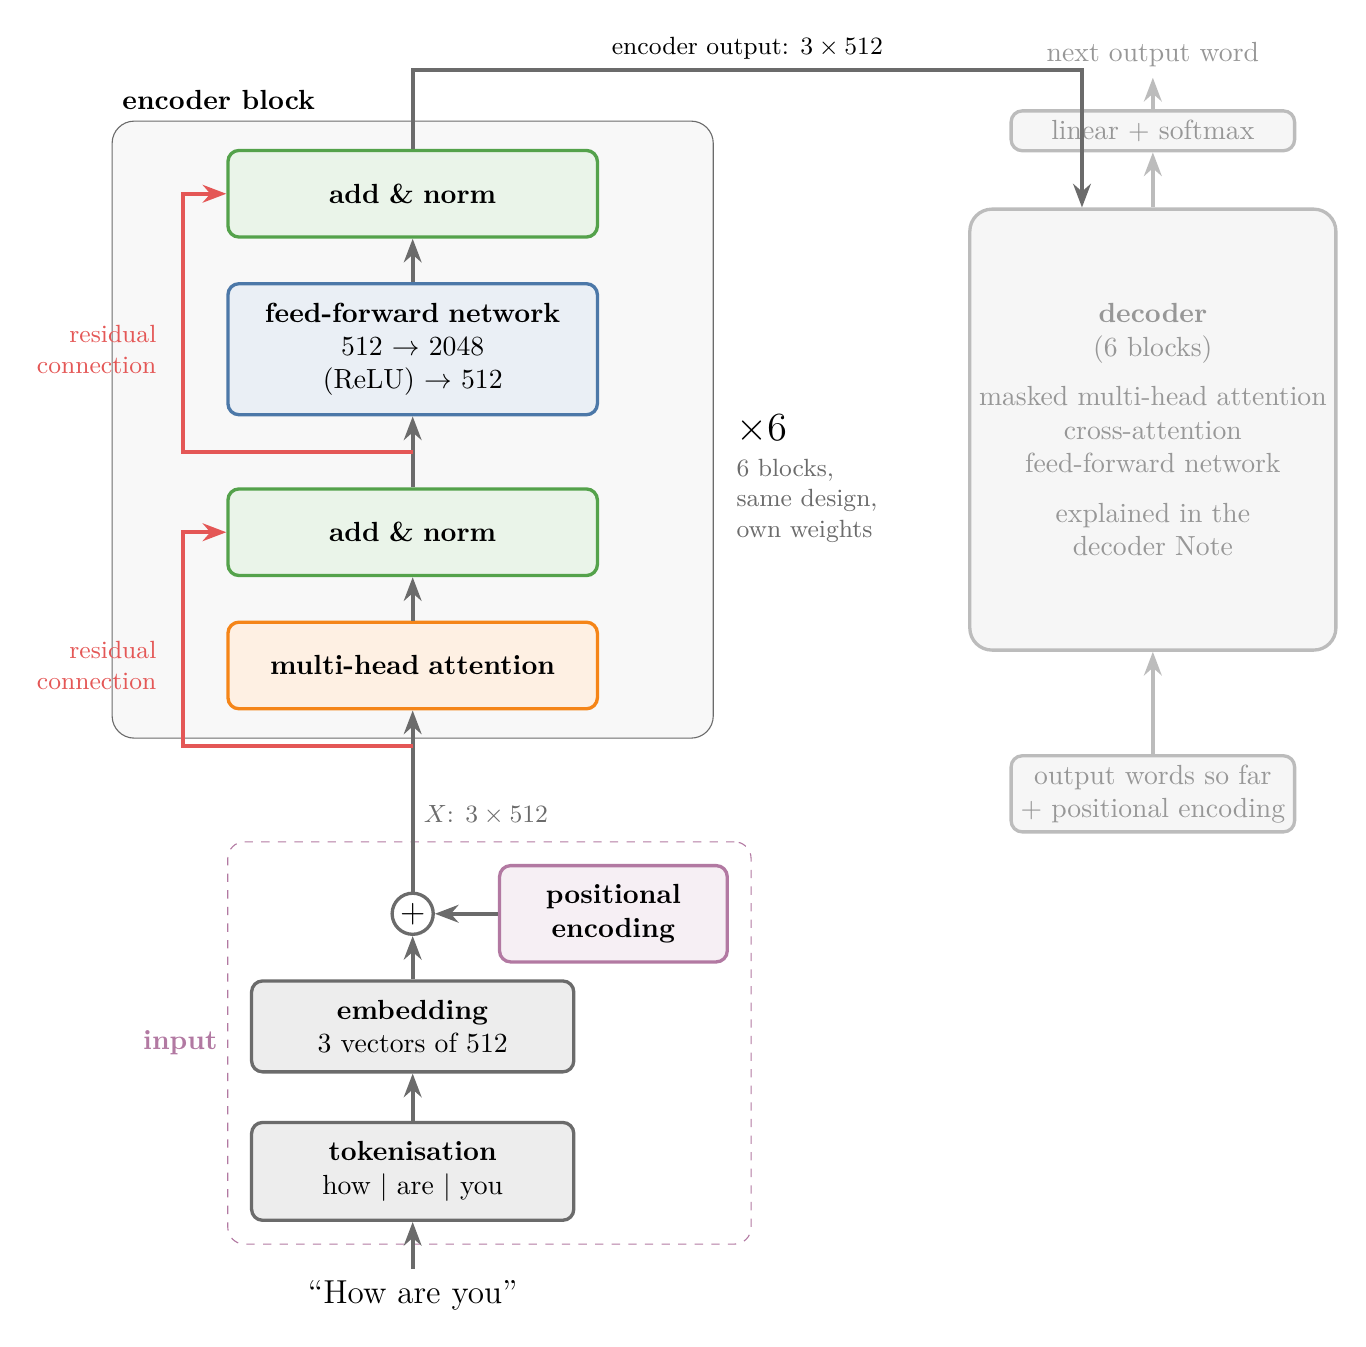
\begin{tikzpicture}[every node/.append style={font=\sffamily}]
  % ---- input block (bottom) ----
  \node[font=\sffamily\large] (sent) at (0,0) {``How are you''};
  \node[box=cgrey, text width=3.6cm, above=0.6cm of sent] (tok) {\textbf{tokenisation}\\how $|$ are $|$ you};
  \node[box=cgrey, text width=3.6cm, above=0.6cm of tok] (emb) {\textbf{embedding}\\3 vectors of 512};
  \node[draw=cgrey, circle, inner sep=1pt, font=\large, above=0.55cm of emb] (plus0) {$+$};
  \node[box=cpurple, text width=2.4cm, right=0.8cm of plus0] (pe) {\textbf{positional}\\\textbf{encoding}};
  \draw[arrow] (sent) -- (tok);
  \draw[arrow] (tok) -- (emb);
  \draw[arrow] (emb) -- (plus0);
  \draw[arrow] (pe) -- (plus0);
  \begin{scope}[on background layer]
    \node[draw=cpurple, dashed, rounded corners=6pt, fit=(tok)(emb)(plus0)(pe), inner sep=8pt,
          label={[cpurple, font=\sffamily\bfseries]left:input}] (inbox) {};
  \end{scope}
  % ---- one encoder block ----
  \node[box=corange, text width=4.2cm, above=2.3cm of plus0] (mha) {\textbf{multi-head attention}};
  \node[box=cgreen, text width=4.2cm, above=0.55cm of mha] (an1) {\textbf{add \& norm}};
  \node[box=cblue, text width=4.2cm, above=0.9cm of an1] (ffn) {\textbf{feed-forward network}\\512 $\to$ 2048 (ReLU) $\to$ 512};
  \node[box=cgreen, text width=4.2cm, above=0.55cm of ffn] (an2) {\textbf{add \& norm}};
  \draw[arrow] (plus0) -- node[pos=0.42, right, font=\sffamily\small, text=cgrey] {$X$: $3 \times 512$} (mha);
  \draw[arrow] (mha) -- (an1);
  \draw[arrow] (an1) -- (ffn);
  \draw[arrow] (ffn) -- (an2);
  % residual connections (left side)
  \coordinate (r1) at ([yshift=-0.45cm]mha.south);
  \draw[arrow, draw=cred] (r1) -| ([xshift=-0.55cm]mha.west) |- (an1.west);
  \coordinate (r2) at ($(an1.north)!0.5!(ffn.south)$);
  \draw[arrow, draw=cred] (r2) -| ([xshift=-0.55cm]ffn.west) |- (an2.west);
  \node[font=\sffamily\small, text=cred, align=right, left=0.75cm of mha.west] {residual\\connection};
  \node[font=\sffamily\small, text=cred, align=right, left=0.75cm of ffn.west] {residual\\connection};
  \begin{scope}[on background layer]
    \node[draw=cgrey, fill=cgrey!5, rounded corners=8pt, fit=(mha)(an2), inner xsep=1.45cm, inner ysep=10pt] (enc) {};
  \end{scope}
  \node[font=\sffamily\bfseries\Large, anchor=west] at ([xshift=0.15cm]enc.east) {$\times 6$};
  \node[font=\sffamily\bfseries, anchor=south west] at (enc.north west) {encoder block};
  \node[font=\sffamily\small, text=cgrey, align=left, anchor=west] at ([xshift=0.15cm, yshift=-0.9cm]enc.east) {6 blocks,\\same design,\\own weights};
  % ---- decoder (greyed) ----
  \node[draw=cgrey!45, fill=cgrey!6, rounded corners=8pt, text=cgrey!70, align=center, minimum width=4.6cm, minimum height=5.6cm,
        font=\sffamily] (dec) at ([xshift=9.4cm]enc.center) {\textbf{decoder}\\(6 blocks)\\[6pt]masked multi-head attention\\cross-attention\\feed-forward network\\[6pt]explained in the\\decoder Note};
  \node[draw=cgrey!45, fill=cgrey!6, rounded corners=4pt, text=cgrey!70, minimum width=3.6cm, above=0.7cm of dec] (lin) {linear + softmax};
  \node[text=cgrey!70, above=0.4cm of lin] (outw) {next output word};
  \node[draw=cgrey!45, fill=cgrey!6, rounded corners=4pt, text=cgrey!70, minimum width=3.6cm, align=center, below=1.3cm of dec] (din) {output words so far\\+ positional encoding};
  \draw[arrow, draw=cgrey!45] (din) -- (dec);
  \draw[arrow, draw=cgrey!45] (dec) -- (lin);
  \draw[arrow, draw=cgrey!45] (lin) -- (outw);
  % encoder output to decoder
  \draw[arrow] (an2.north) -- ++(0,1.0) -| node[pos=0.25, above, font=\sffamily\small] {encoder output: $3 \times 512$} ([xshift=-0.9cm]dec.north) ;
\end{tikzpicture}
\end{document}
